\documentclass[dvipdfmx]{jsarticle}
\usepackage[dvipdfmx]{hyperref, xcolor, graphicx}
\hypersetup{
    colorlinks=true,
    citecolor=blue,
    linkcolor=blue,
    urlcolor=blue,
}

% 数式
\usepackage{amsmath,amsfonts,amssymb,amsthm, mathtools}
\usepackage{bm}
\usepackage{physics}
\usepackage{tcolorbox}
\tcbuselibrary{breakable} % 必要に応じて

\newtcolorbox{mybox}[1][]{%
  title=#1,
  fonttitle=\gtfamily\sffamily\bfseries,
  colframe=blue,
  colback=blue!3!,
  breakable, % 長文対応したい場合
}

\usepackage[dvipdfmx]{graphicx}
\usepackage{tikz} %図を描く
\usetikzlibrary{positioning, intersections, calc, arrows.meta,math} 

\usepackage{here}

\begin{document}

\section{なんで分配関数を計算するのか?}
第三章では、(正規化された)分配関数$Z_n^{(0)}(\beta)$の$n\to\infty$極限での振る舞いを調べるのだが、ベイズ統計の枠組みにおいてこのような量を計算する理由がわかりにくい。
この資料では、分配関数の計算がなぜ必要なのかを説明する。分配関数は
\begin{equation}
    Z_n^{(0)}(\beta) \coloneqq \int\exp(-n\beta K_n(w))\varphi(w)\,dw
\end{equation}
と定義される。$K_n(w)$は経験誤差関数と呼ばれる量であり、
\begin{equation}
    K_n(w) \coloneqq -\frac{1}{n}\sum_{i=1}^n f(X_i, w) = -\frac{1}{n}\sum_{i=1}^n \ln \frac{p(X_i|w_0)}{p(X_i|w)}
\end{equation}
である。パラメータ$w$が確率変数であることから、$K_n(w)$も確率変数となる。

\begin{mybox}[事後分布による期待値計算と分配関数]
    分配関数の振る舞いを解明することは、事後分布による積分計算の挙動を解明することと等価である。
    なぜなら、事後分布$p(w|X^n)$は
    \begin{equation}
        p(w|X^n) \propto \varphi(w)\prod_{i=1}^{n}p(X_i|w)^{\beta} \propto \varphi(w)\exp(-n\beta K_n(w))
    \end{equation}
    と変形できるためである。仮に$K_n(w)$が$w=w_0$で唯一の極小値を持っているとすると、期待値計算では$w=w_0$近傍の値が主要な寄与を持つことになる。
    第三章の前半では、このような予想が実際に成り立つことを示し、$w_0$近傍以外の効果がどれくらいのオーダーで$0$に収束するかを調べる。
\end{mybox}

第三章の前半は、汎化損失$G_n$を求めるために必要な事後分布による期待値計算について、Gauss積分で近似できること(鞍点近似を適用できること)を示すことが目的だと思われる。
$K_n(w)$の確率的な振る舞い(すなわち$f(X, w)$の確率的な振る舞い)を調べることで、鞍点近似の妥当性の評価を行う。


\begin{mybox}[三章前半のゴール]
汎化損失$G_n$が$n\to\infty$の極限で以下の振る舞いをする:
\begin{equation}
    G_n = L(\omega_0) + \frac{1}{n}\qty(\frac{d}{2\beta} + \frac{1}{2}\abs{\xi}^2 - \frac{1}{2\beta}\tr(IJ^{-1})) + \mathrm{o_p}\qty(\frac{1}{n})\;。
\end{equation}
\end{mybox}
ここで汎化損失$G_n$はどのような量と結びついていたかを復習する。確率変数$f(w)$に対して、事後分布による期待値を
\begin{equation}
    \ev{f(w)}_{w|X^n} \coloneqq \int f(w) p(w|X^n)\,dw
\end{equation}
と定義する。このとき、汎化損失は以下のように表される:
\begin{equation}
    G_n = -\mathbb{E}_X\qty[\ln(\ev{p(X|w)}_{w|X^n})]\;。
    \label{eq:gn1}
\end{equation}
分配関数の計算を行うことができれば、$\ev{f(X,w)}_{w|X^n}$の振る舞い、すなわち$\ev{p(X|w)}_{w|X^n}$の振る舞いを直接評価できる。
しかし、それが対数関数の中に入っているため、$G_n$を直接計算することは難しそうだ。
途中まで計算を進めてみると、
\begin{align}
    G_n &= -\mathbb{E}_X\qty[\ln(\ev{p(X|w)}_{w|X^n})] = -\mathbb{E}_X\qty[\ln{p(X|w_0)} - \ln\ev{\frac{p(X|w_0)}{p(X|w)}}_{w|X^n}] \notag \\
    &= -\mathbb{E}_X\qty[\ln(p(X|w_0))] + \mathbb{E}_X\qty[\ln\ev{e^{f(X,w)}}_{w|X^n}] 
\end{align}
という形になる。右辺第一項は$L(w_0)$そのものである。第二項の計算が難しいのだが、ログをなくすためにはTaylor展開$\ln(1+x) = x - x^2/2 + \cdots$を適用すれば良いことに気づく。
確率変数$X$に対して、$X^2$までの項の寄与を考えると
\begin{equation}
    \ln\ev{e^X} = \ln\ev{1+X + \frac{X^2}{2}} = \ev{X + \frac{X^2}{2}} - \frac{1}{2}\ev{X+\frac{X^2}{2}}^2
    = \ev{X} + \frac{1}{2}\qty(\ev{X^2} - \ev{X}^2)
\end{equation}
が成り立つので、
\begin{equation}
    \ln\ev{e^{f(X,w)}}_{w|X^n} = \ev{f(X,w)}_{w|X^n} + \frac{1}{2}\mathbb{V}[f(X,w)]
    \label{eq:taylor}
\end{equation}
という形になる。$\mathbb{V}[f(X,w)]$は分散である。
次章で示すのだが、$G_n = -\mathcal{G}_n(1)$の関係式を用いた計算は、上記のTaylor展開を用いた計算と全く同じ結果を得るらしい。その結果を先に述べておく:
\begin{equation}
    G_n = L(w_0) + \frac{1}{n}\qty(\ev{nK(w)}_{w|X^n} - \frac{1}{2}\mathbb{E}_X\qty[\mathbb{V}[nf(X,w)]]) + \mathrm{o_p}\qty(\frac{1}{n})\;。
\end{equation}
ここで
\begin{equation}
    K(w) = \mathbb{E}_X\qty[f(X,w)],\qquad \mathbb{V}[f(X,w)] = \ev{f(X,w)^2}_{w|X^n} - \ev{f(X,w)}_{w|X^n}^2
\end{equation}
であるため、$\mathcal{G}_n(1)$を用いた計算は式\eqref{eq:taylor}と同じ形(なぜか分散の符号が逆)になっている。
さて、ここまで計算できれば、あとは$f(X,w)$の確率的な振る舞いがどのようなものかを解析すれば良い。

\section{Taylor展開の正当化}
上で行ったTaylor展開は、第二章で得られた結果を再現しているようである。
第二章で議論したように、とある性質の良い関数$\mathcal{G}_n(\alpha)$を用いて
\begin{equation}
    G_n = -\mathcal{G}_n(1)
\end{equation}
と計算できることがわかっている。しかし、$\mathcal{G}_n(1)$の値を直接計算することは難しい。
そこで、$\alpha=0$周りのTaylor展開を考えると、一般の$\alpha$に対して
\begin{equation}
    \mathcal{G}_n(\alpha) = \mathcal{G}_n(0) + \sum_{k=1}^{\infty} \frac{1}{n!}\mathcal{G}_n^{(k)}(0)(\alpha - 0)^k
\end{equation}
と表される(と$\mathcal{G}$に仮定を置いている)。ただし、$\mathcal{G}_n^{(k)}$は$\mathcal{G}_n$の$\alpha$による$k$階微分である。
また、$\mathcal{G}_n(0) = 0$となることは簡単に示せる。正則理論の枠組み
\footnote{事後分布が正規分布で近似できるという特別な場合の理論であり、具体的には3つの仮定を置くことで成り立つ:
    \begin{enumerate}
        \item 真の分布に対して最適なパラメータが一つである。すなわち、$W_0 = \{w_0\} \subset W$である。 
        \item $L(w)$は、そのHessianが$w=w_0$で正定値行列となる。
        \item サンプルの数(データセットの数)$n$が非常に大きい。非常に大きいとは、確率過程$\eta_n(w)$が法則収束しているとみなせる程度の大きさである。
    \end{enumerate}
}
を考えている範囲では、高次の微分項がほとんどゼロになることが示される:
\begin{equation}
    \forall k \geq 3, \quad \abs{\mathcal{G}_n^{(k)}(0)} = \mathrm{o_p}\qty(\frac{1}{n})\;。
\end{equation}
したがって、
\begin{equation}
    G_n = -\mathcal{G}_n(1) = -\mathcal{G}_n^{(0)}(0) - \frac{1}{2}\mathcal{G}_n^{(1)}(0) + \mathrm{o_p}\qty(\frac{1}{n})\;。
    \label{eq:gn2}
\end{equation}
という関係式を用いて$G_n$を求められる。さらに任意の$k$について、$\mathcal{G}_n^{(k)}(0)$は
\begin{equation}
    l_k(X) \coloneqq \ev{(\ln{p(X|w)})^k}_{w|X^n} = (-1)^k\ev{\qty(f(X,w) - \ln{p(X|w_0)})^k}_{w|X^n}
\end{equation}
で定義される$l_k(X)$を用いて計算可能である。これを用いると、
\begin{align}
    \mathcal{G}_n^{(1)}(0) &= \mathbb{E}_X\qty[\ev{f(X,w)}_{w|X^n}] \\
    \mathcal{G}_n^{(2)}(0) &= \mathbb{E}_X\qty[\mathbb{V}[f(X,w)]] \\
\end{align}
となる。したがって式\eqref{eq:gn2}の右辺を計算すると、
\begin{equation}
    G_n = L(w_0) + \frac{1}{n}\qty(\ev{nK(w)}_{w|X^n} - \frac{1}{2}\mathbb{E}_X\qty[\mathbb{V}[nf(X,w)]]) + \mathrm{o_p}\qty(\frac{1}{n})
\end{equation}
という結果を得る。これは式\eqref{eq:taylor}と(分散の符号を除いて)同じである。

\section{分配関数の計算}
$G_n$を計算するために最後に必要なことは、$f(X,w)$の確率的な振る舞いを明らかにすることである。
そのためには、事後分布による積分を楽に評価できるようにする必要がある。

\begin{equation}
    p(w|X^n) \propto \varphi(w)\exp(-n\beta K_n(w))
\end{equation}
であったため、分配関数
\begin{equation}
    Z_n^{(0)}(\beta) = \int\exp(-n\beta K_n(w))\varphi(w)\,dw
\end{equation}
の性質を明らかにすれば、期待値計算を評価できると考えられる。積分をサボりたいため、被積分関数の寄与が最も大きい部分、すなわち
\begin{equation}
    \omega^* = \arg\min_{w} K_n(w) = \arg\min_{w} L(w) = w_0
\end{equation}
の$\epsilon\text{-}$近傍を考えてみよう。正則理論の枠組みでは、
\begin{equation}
    \left.\laplacian{K_n(w)}\right|_{w=w_0}
\end{equation}
が正定値行列という仮定を入れていた。したがって図\ref{fig:spiky-kn}のような状況になっており、$w_0$の$\epsilon\text{-}$近傍が最も積分に寄与する。
実際に、$\epsilon\text{-}$近傍の外側の寄与はほとんどないことが示される。
さらに、$\epsilon\text{-}$近傍の内側では、被積分関数をGaussianとして扱えることが示されるため、$\mathbb{R}^d$全体の積分に置き換えて、解析的に計算できるようになる。
これが分配関数の計算ストーリーである。

\begin{figure}[H]
\centering
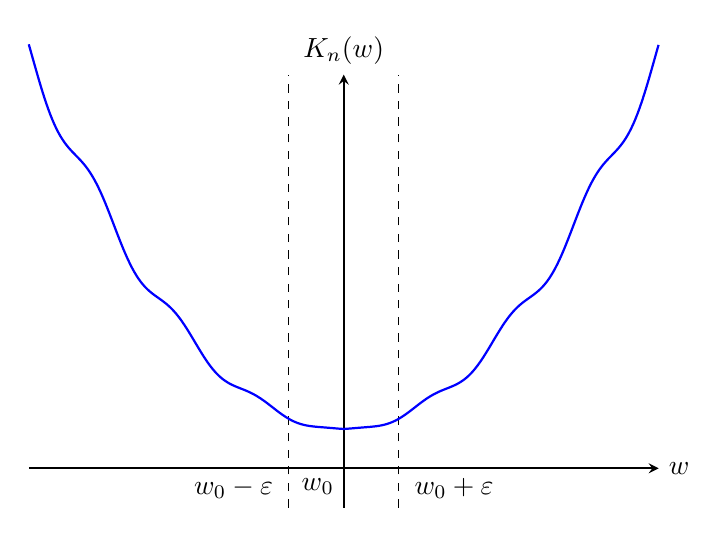
\begin{tikzpicture}[samples=300,domain=-4:4]
    % epsilon
    \def\eps{0.7} % εの大きさ

    % 軸
    \draw[->,>=stealth,semithick] (-4,0)--(4,0) node[right]{$w$}; 
    \draw[->,>=stealth,semithick] (0,-0.5)--(0,5.0) node[above]{$K_n(w)$}; 
    \draw (0,0) node[below left]{$w_0$};

    % ε近傍の塗りつぶし(灰色、半透明)
    \draw[dashed] (-\eps, -0.5) -- (-\eps, 5.0);
    \draw[dashed] (\eps, -0.5) -- (\eps, 5.0);
    \node[below] at (-2*\eps, 0) {$w_0 - \varepsilon$};
    \node[below] at (2*\eps, 0) {$w_0 + \varepsilon$};

    % 関数
    \draw[thick,blue] plot (\x, 
        {0.3*(\x)^2 + 0.05*abs(\x)*cos(6 * \x * 180 / pi) + 0.5});
\end{tikzpicture}
\caption{関数 $K_n(w)$ とその極小点 $w_0$ の $\varepsilon\text{-}$近傍}
\label{fig:spiky-kn}
\end{figure}

\section{分配関数の計算のイメージ}
積分を一番サボる方法は、被積分関数が最も大きい場所に対する短冊近似(抜き出す区間を$\varDelta_n(w_0)$とする。この区間は関数のピーキー性を見ながら調節する必要があるため、$n$に依存して良い)を実行することである:
\begin{equation}
    Z_n^{(0)}(\beta) = \int\exp(-n\beta K_n(w))\varphi(w)\,dw \approx \underbrace{\exp(-n\beta K_n(w_0))}_{=1}\varphi(w_0)\varDelta_n(w_0)
\end{equation}
しかしこれでは精度が悪すぎて、$n$に対する振る舞いの情報が落ちてしまっている。$n\to\infty$に近づくにつれてどのような挙動をするか見たいので、少しだけ$w_0$周りの寄与を足すことにする。
これが第三章で行っている鞍点近似のお気持ちである。その結果として、
\begin{equation}
    Z_n^{(0)}(\beta) \approx \exp(\frac{\beta}{2}\abs{\xi_n}^2)\varphi(w_0)\underbrace{\qty(\frac{2\pi}{n\beta})^{d/2}\det{J}^{-1/2}}_{=\varDelta_n(w_0)}
\end{equation}
という形になる。確率変数$\xi_n$は$n\to\infty$で$0$に確率収束するような性質を持っている(これが大事なのに地味に示せない。。。)ため、
\begin{equation}
    Z_n^{(0)}(\beta) \approx \qty[1+\underbrace{\frac{\beta}{2}\abs{\xi_n}^2+\cdots}_{\to 0\,(n\to\infty)}]\varphi(w_0)\varDelta_n(w_0)
\end{equation}
となり、$n\to\infty$の極限で短冊近似の結果を再現する。


\section{第三章の主要な結果}
第三章で得られる最も主要な主張はおそらく、正則理論の仮定のもとでは事後分布が正規分布で近似できる(正規分布に法則収束する)ということである。
なぜなら、ベイズ理論の目的は$G_n$を計算することであり、$G_n$は事後分布の期待値計算を用いて計算できるからである。
\begin{mybox}[事後分布が正規分布に法則収束する]
    正則理論の仮定の元では、事後分布$p(w|X^n)$は、$J=\laplacian L(w_0)$を用いて、平均$\omega_0$、分散$(nJ)^{-1}$の正規分布に法則収束する:
\begin{equation}
    p(w|X^n) \xrightarrow[n\to\infty]{\mathrm{d}} \mathcal{N}(\omega_0, (nJ)^{-1})
    = \frac{1}{\sqrt{(2\pi)^{d}\det{(nJ)^{-1}}}}\exp(\frac{1}{2}(\omega-\omega_0)^{\top}nJ(\omega-\omega_0))\;。
\end{equation}
\end{mybox}
この結果に関連する議論をしているのが3.4節までである。
3.5節では、ベイズ推測以外の方法(事後確率最大化法、最尤推定法、平均プラグイン法)を用いた場合の$f(X,w)$の振る舞いを調べているようだった。
3.6節では、事後分布が正規分布で近似できるという仮定の元で、サンプルだけから汎化損失$G_n$を数値的に推定する方法を示している。

\begin{mybox}[サンプルだけから汎化損失を推定する]
    汎化損失はその定義から、サンプルだけでは計算することができないが、サンプルだけから計算可能な正則の情報量基準を
    \begin{equation}
        \text{RIC} \coloneqq T_n + \frac{1}{n}\tr(IJ^{-1})
    \end{equation}
    と定義すると、$G_n - L(w_0)$と$\text{RIC} - L_n(w_0)$は平均と分散が漸近的に一致することが示される。
    後者の値はサンプルだけから計算できるため、汎化損失の推定値として用いることができる。(たぶん)
\end{mybox}



\end{document}
